%\begin{figure*}[h]
%    \caption{Example of a parametric plot ($\sin (x), \cos(x), x$)}
%    \centering
%    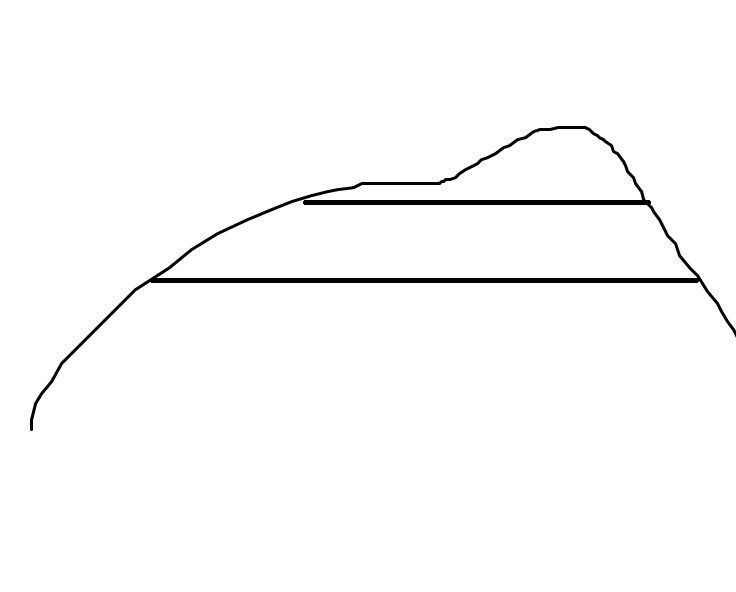
\includegraphics[width=0.5\textwidth]{graphic_example}
%\end{figure*}

\subsection{Introduction}

We want to generalize the notion of the \textit{length} towards all 
the subsets of $\mathbb{R}$.
Such a generalized function is usually called \textit{measure}.
But, unfortunately, such a function does not exist.

\begin{theorem}
\label{the:measureNotExists}
    There exist no such function $\mu: 2^{[0,1]} \to [0, +\infty)$ that satisfies the 
    following properties:
    \begin{enumerate}
        \item {
            The function is non-negative;
        }
        \item {
            It's countably additive;
        }
        \item {
            It's monotonic: the measure of a subset is not greater than the entire set;
        }
        \item {
            Translation does not change the measure;
        }
        \item {
            The measure of the unit interval is 1.
        }
    \end{enumerate}
\end{theorem}

\begin{proof}
    First, several definitions:
    \begin{enumerate}[label={Step \arabic*.}]
        \item {
            Let's define the following equivalence relation:
            if $x$, $y$ are from the unit interval, we'll say that
            $x \sim y$ if $x - y \in \mathbb{Q}$.
        }
        \item {
            Let's choose $N \subset [0, 1/3]$ such that it contains
            \textit{precisely one} element from each equivalence class.
            (Such an $N$ exists if the axiom of choice holds true).
        }
        \item {
            For all $r \in \mathbb{Q}$ define $N_r = N + r$.
        }
    \end{enumerate}

    \begin{itemize}%[font={\bfseries}]
        \item[Claim 1.] {
            The sets $N_R$ are congruent to $N$ and are pairwise disjoint.
        }
        \item[Proof.] {
            The sets are congruent by definition. Let's prove that 
            they are pairwise disjoint.

            Assume that $x \in N_{r_1} \cap N_{r_2}$ for some
            $r_1, r_2 \in \mathbb{Q}$.
            Then $x - r_1 \in N$, $x - r_2 \in N$, but
            $(x - r_1) \sim (x - r_2) \implies r_1 = r_2$.
        }
        \item[Claim 2.] {
            \[
                \Bigl[\frac{1}{3}, \frac{2}{3}\Bigr] \in
                \bigcup_{r \in \mathbb{Q} \cap [0, 2/3]} N_r
            \]
        }
        \item[Proof.] {
            If $x \in [1/3, 2/3]$, then
            $\exists!\, y \in N$ such that $x = y + q$ for some $q \in \mathbb{Q}$,
            as $N$ contains exactly one representative from each of the equivalence classes.
            It is easy to see that such $q \in [0, 2/3]$.
        }
    \end{itemize}

    We arrive at the following conclusion:
    \[
        \frac{1}{3} = \mu\bigl([1/3, 2/3]\bigr) \le \mu\Bigl( \bigcup_{r \in \mathbb{Q} \cap [0, 2/3]} N_r \Bigr) = 
        \sum_{r \in \mathbb{Q} \cap [0, 2/3]} \mu(N_r) \le 1
    \]
    What is $\mu(N)$ then? If $\mu(N) = 0$, then 
    \[
        \mu\Bigl( \bigcup_{r \in \mathbb{Q} \cap [0, 2/3]} N_r \Bigr) = 
        \sum 0 = 0
    \]
    If $\mu(N) = \varepsilon > 0$, then the sum is $+\infty$. 
    But it's supposed to be in $[1/3, 1]$?!
\end{proof}

\begin{consequence}
    We cannot generalize the notion of length to all subsets of real numbers.
\end{consequence}

\subsection{Lebesgue Outer Measure}
\begin{definition}
    If $I \subset \mathbb{R}$ is an interval, then
    $l(I) = \text{the length of $I$}$. If $I$ is unbounded, then $l(I) = \infty$.
\end{definition}
\begin{definition}[Outer Measure]
    \begin{align*}
        &
        m^* : 2^{\mathbb{R}} \to [0, +\infty]
        \\&
        m^*(A) = \inf \Bigl\{ \sum_{j = 1}^{\infty} l(I_j) \mid 
        I_j \text{ --- open intervals},\ A \subseteq \bigcup_{j=1}^{\infty} I_j\Bigr\}
    \end{align*}
    In words, it's the infimum of all \textit{countable} covers of $A$.
    (A countable sum either converges or diverges to infinity).
\end{definition}
\begin{remark}
    This is certainly not a measure --- otherwise, it would contradict Theorem~\ref{the:measureNotExists}.
\end{remark}

\begin{example}
    If $A$ is countable, then $m^*(A) = 0$.
\end{example}
\begin{proof}
    Let's choose an arbitrary $\varepsilon > 0$ and prove that $m^*(A) \le 2\varepsilon$.
    Let's choose a cover of the points with segments of lengths $\varepsilon$, $\varepsilon / 2$, $\varepsilon / 2^2$, and so on.
    Then \[
        m^*(A) = \inf \{\dots\} \le \varepsilon + \frac{\varepsilon}{2} + \frac{\varepsilon}{2^2} + \dots = 2\varepsilon
    \]
\end{proof}

\begin{proposition}
    If $A$ is an interval, then $m^*(A) = l(A)$.
\end{proposition}
\begin{proof}
    \begin{enumerate}[label=\alph*)]
        \item {
            $A$ is a closed interval, $A = [a, b]$.
            \begin{enumerate}[label=\arabic*.]
                \item {
                    $m^*(A) \le b - a$.
                    To prove this, we can cover $A$ with a single interval:
                    \[ (a - \varepsilon, b + \varepsilon) \implies \sum l(I_j) = b - a + 2\varepsilon \]
                    Now take $\varepsilon \to 0$.
                }
                \item {
                    $m^*(A) \ge b - a$.
                    Suppose we an infinite cover of $A$ by open intervals.
                    Since $A$ is a compact set, we can choose a finite subcover.
                    The case of a finite cover with open intervals is obvious.
                }
            \end{enumerate}
        }
        \item {
            If $A$ is an open or semiclosed interval, we can approximate it from both sides
            by closed intervals.
        }
        \item {
            If $A$ is unbounded, then all of the covers would have infinite sum, and thus 
            the infimum will be infinite as well.
        }
    \end{enumerate}
\end{proof}